
\subsection*{Introducción}
\begin{wrapfigure}{L}{0.4\textwidth}
	\begin{center}
		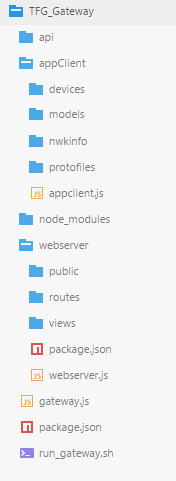
\includegraphics[width=0.3\textwidth]{graphs/estructuraServidor.png}
	\end{center}
	\caption{Estructura del directorio del servidor}
	\label{fig:estructuraServidor}
\end{wrapfigure}

El servidor se puede dividir en dos partes \textit{Front-end} y \textit{Back-End} que son términos que se refieren a la separación entre una capa de presentación y una capa de acceso a datos respectivamente. 

\subsection*{Estructura del servidor}

El servidor está compuesto por el directorio que se observa en la figura \ref{fig:estructuraServidor} y a continuación se describe la función de cada directorio:


\begin{description}
	\item[api: ] en este directorio se encuentran las definiciones de llamadas REST al servidor.
	\item[appClient: ] Esta carpeta contiene el \textit{Back-end} de la web:
	\begin{description}
		\item[devices: ] se definen las funciones relacionadas con la gestión de los nodos.
		\item[models: ] aquí se definen los modelos para guardarlos en la base de datos.
		\item[nwkinfo: ] se definen las funciones relacionadas con la gestión del concentrador.
		\item[protofiles: ] aquí se almacenan los ficheros .proto de \textit{Protocol Buffers}.
		\item[appClient.js: ] en este fichero se inicia el servidor que se comunica con el concentrador y se procesan los mensajes.
	\end{description}
	\item[node\_modules: ] librerías utilizadas en el proyecto.
	\item[webserver: ] en este directorio está contenida la lógica del \textit{Front-end}:
	\begin{description}
		\item[public: ] interfaz del cliente en AngularJS.
		\item[routes: ] Definición de rutas.
		\item[views: ] archivos html de las vistas.
		\item[webserver.js: ] se inicia el cliente y se gestiona las peticiones a la web por parte del usuario.
	\end{description}
	\item[gateway.js: ] inicia el \textit{back-end} y el \textit{front-end} y la comunicación entre ambas por \textit{web-sockets}.
	\item[run\_gateway.sh: ] \textit{script} para iniciar el servidor.
\end{description}

\subsection*{Back-end}

El \textit{Back-end} es el área que se dedica a la lógica, en este encontramos una interfaz que se encarga de comunicarse con el concentrador y otra que se encarga de comunicarse con el \textit{Front-end} usando \textit{Web-Sockets}.


Al inicio del archivo \textit{appClient.js} se abre el puerto 3000 y se mantiene a la escucha hasta que el concentrador se conecta. Cuando el concentrador se conecta, este el envía la información de configuración. \\

Toda la información de la red se almacena en una base de datos MongoDB\R, también se almacena los datos enviados por los nodos así como sus parámetros de configuración.\\

Una vez la conexión entre el concentrador y el \textit{back-end} se ha establecido, ambos se quedan a la espera de que el usuario desde el \textit{front-end} permita la conexión de los nodos a la red.


\sectionx{Front-end}

El \textit{Front-end} es la interfaz del servidor con el usuario. Para facilitar el control de las vistas se ha utilizado el \textit{framework AngularJS}.\\

Angular es un \textit{framework} \ac{MVC} para la construcción de aplicaciones de una única página del lado del cliente en HTML y JavaScript.\\

Como se ha mencionado anteriormente, el patrón que se usa en Angular es el conocido como Modelo, Vista y Controlador:

\begin{description}
	\item[Vistas: ] Será el código HTML y todo lo que presente los datos o información.
	\item[Controladores: ] Se encarga de toda la lógica de la aplicación.
	\item[Modelo: ] El modelo es la estructura que define un tipo de dato, y permite acceder a él en la base de datos.
\end{description}


